\chapter{Bayesian statistics}


\section{Introduction}
Using the posterior distribution to summarize everything we know about a set of unknown variables is at the core of Bayesian statistics. In this chapter, we discuss this approach to statistics in more detail.


\section{Summarizing posterior distributions}
The posterior $p(\vec{\theta}|\mathcal{D})$ summarizes everything we know about the unknown quantities $\vec{\theta}$. In this section, we discuss some simple quantities that can be derived from a probability distribution, such as a posterior. These summary statistics are often easier to understand and visualize than the full joint.


\subsection{MAP estimation}
We can easily compute a \textbf{point estimate} of an unknown quantity by computing the posterior mean, median or mode. In Section \ref{sec:Bayesian-decision-theory}, we discuss how to use decision theory to choose between these methods. Typically the posterior mean or median is the most appropriate choice for a realvalued quantity, and the vector of posterior marginals is the best choice for a discrete quantity. However, the posterior mode, aka the MAP estimate, is the most popular choice because it reduces to an optimization problem, for which efficient algorithms often exist. Futhermore, MAP estimation can be interpreted in non-Bayesian terms, by thinking of the log prior as a regularizer (see Section TODO for more details).

Although this approach is computationally appealing, it is important to point out that there are various drawbacks to MAP estimation, which we briefly discuss below. This will provide motivation for the more thoroughly Bayesian approach which we will study later in this chapter(and elsewhere in this book).


\subsubsection{No measure of uncertainty}
The most obvious drawback of MAP estimation, and indeed of any other \emph{point estimate} such as the posterior mean or median, is that it does not provide any measure of uncertainty. In many applications, it is important to know how much one can trust a given estimate. We can derive such confidence measures from the posterior, as we discuss in Section \ref{sec:Credible-intervals}.

\subsubsection{Plugging in the MAP estimate can result in overfitting}
If we don’t model the uncertainty in our parameters, then our predictive distribution will be overconfident. Overconfidence in predictions is particularly problematic in situations where we may be risk averse; see Section \ref{sec:Bayesian-decision-theory} for details.

\subsubsection{The mode is an untypical point}
Choosing the mode as a summary of a posterior distribution is often a very poor choice, since the mode is usually quite untypical of the distribution, unlike the mean or median. The basic problem is that the mode is a point of measure zero, whereas the mean and median take the volume of the space into account. See Figure \ref{fig:untypical-point}.

\begin{figure}[hbtp]
\centering
\subfloat[]{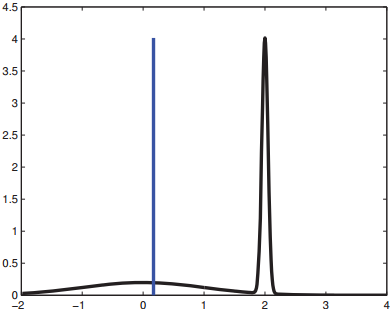
\includegraphics[scale=.50]{untypical-point-a.png}} \\
\subfloat[]{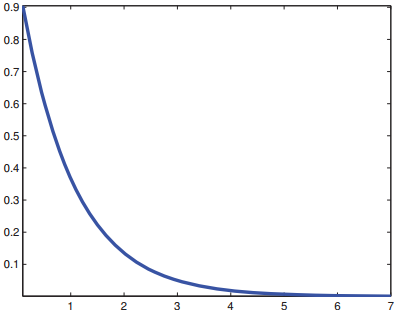
\includegraphics[scale=.50]{untypical-point-b.png}}
\caption{(a) A bimodal distribution in which the mode is very untypical of the distribution. The thin blue vertical line is the mean, which is arguably a better summary of the distribution, since it is near the majority of the probability mass. (b) A skewed distribution in which the mode is quite different from the mean.}
\label{fig:untypical-point} 
\end{figure}

How should we summarize a posterior if the mode is not a good choice? The answer is to use decision theory, which we discuss in Section \ref{sec:Bayesian-decision-theory}. The basic idea is to specify a loss function, where $L(\theta,\hat{\theta})$ is the loss you incur if the truth is $\theta$ and your estimate is $\hat{\theta}$. If we use 0-1 loss $L(\theta,\hat{\theta})=\mathbb{I}(\theta \neq \hat{\theta})$(see section \ref{sec:Loss-function-and-risk-function}), then the optimal estimate is the posterior mode. 0-1 loss means you only get “points” if you make no errors, otherwise you get nothing: there is no “partial credit” under this loss function! For continuous-valued quantities, we often prefer to use squared error loss, $L(\theta,\hat{\theta})=(\theta-\hat{\theta})^2$ ; the corresponding optimal estimator is then the posterior mean, as we show in Section \ref{sec:Bayesian-decision-theory}. Or we can use a more robust loss function, $L(\theta,\hat{\theta})=|\theta-\hat{\theta}|$, which gives rise to the posterior median.

\subsubsection{MAP estimation is not invariant to reparameterization *}
A more subtle problem with MAP estimation is that the result we get depends on how we parameterize the probability distribution. Changing from one representation to another equivalent representation changes the result, which is not very desirable, since the units of measurement are arbitrary (e.g., when measuring distance, we can use centimetres or inches).

To understand the problem, suppose we compute the posterior forx. If we define y=f(x), the distribution for yis given by Equation \ref{eqn:General-transformations}. The $\frac{\mathrm{d}x}{\mathrm{d}y}$ term is called the Jacobian, and it measures the change in size of a unit volume passed
through $f$. Let $\hat{x}=\arg\max_x p_x(x)$ be the MAP estimate for $x$. In general it is not the case that $\hat{x}=\arg\max_x p_x(x)$ is given by $f(\hat{x})$. For example, let $X \sim \mathcal{N}(6,1)$ and $y=f(x)$, where $f(x)=1/(1+\exp(-x+5))$. 

\begin{figure}[hbtp]
\centering
    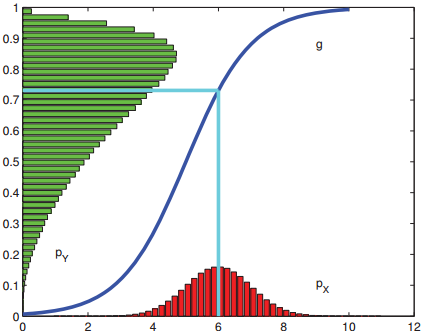
\includegraphics[scale=.70]{mode-reparameterization.png}
\caption{Example of the transformation of a density under a nonlinear transform. Note how the mode of the transformed distribution is not the transform of the original mode. Based on Exercise 1.4 of (Bishop 2006b).}
\label{fig:mode-reparameterization} 
\end{figure}

We can derive the distribution of $y$ using Monte Carlo simulation (see Section \ref{sec:Monte-Carlo-approximation}). The result is shown in Figure \ref{sec:mode-reparameterization}. We see that the original Gaussian has become “squashed” by the sigmoid nonlinearity. In particular, we see that the mode of the transformed distribution is not equal to the transform of the original mode.

The MLE does not suffer from this since the likelihood is a function, not a probability density. Bayesian inference does not suffer from this problem either, since the change of measure is taken into account when integrating over the parameter space.


\subsection{Credible intervals}
\label{sec:Credible-intervals}
In addition to point estimates, we often want a measure of confidence. A standard measure of confidence in some (scalar) quantity $\theta$ is the “width” of its posterior distribution. This can be measured using a $100(1−\alpha)\%$ credible interval, which is a (contiguous) region $C=(\ell,u)$(standing for lower and upper) which contains $1−\alpha$ of the posterior probability mass, i.e.,
\begin{equation}
C_{\alpha}(\mathcal{D}) \quad \text{where } P(\ell \leq \theta \leq u)=1-\alpha
\end{equation}

There may be many such intervals, so we choose one such that there is $(1−\alpha)/2$ mass in each tail; this is called a \textbf{central interval}.

If the posterior has a known functional form, we can compute the posterior central interval using $\ell=F^{-1}(\alpha/2)$ and $u=F^{-1}(1-\alpha/2)$, where $F$ is the cdf of the posterior. 

If we don’t know the functional form, but we can draw samples from the posterior, then we can use a Monte Carlo approximation to the posterior quantiles: we simply sort the $\mathcal{S}$ samples, and find the one that occurs at location $\alpha/\mathcal{S}$ along the sorted list. As $\mathcal{S} \rightarrow \infty$, this converges to the true quantile. 

People often confuse Bayesian credible intervals with frequentist confidence intervals. However, they are not the same thing, as we discuss in Section TODO. In general, credible intervals are usually what people want to compute, but confidence intervals are usually what they actually compute, because most people are taught frequentist statistics but not Bayesian statistics. Fortunately, the mechanics of computing a credible interval is just as easy as computing a confidence interval. 


\subsection{Inference for a difference in proportions}
Sometimes we have multiple parameters, and we are interested in computing the posterior distribution of some function of these parameters. For example, suppose you are about to buy something from Amazon.com, and there are two sellers offering it for the same price. Seller 1 has 90 positive reviews and 10 negative reviews. Seller 2 has 2 positive reviews and 0 negative reviews. Who should you buy from?\footnote{This example is from \url{http://www.johndcook.com/blog/2011/09/27/bayesian-amazon/}}.

On the face of it, you should pick seller 2, but we cannot be very confident that seller 2 is better since it has had so few reviews. In this section, we sketch a Bayesian analysis of this problem. Similar methodology can be used to compare rates or proportions across groups for a variety of other settings.

Let $\theta_1$ and $\theta_2$ be the unknown reliabilities of the two sellers. Since we don’t know much about them, we’ll endow them both with uniform priors, $\theta_i \sim \text{Beta}(1,1)$. The posteriors are $p(\theta_1|\mathcal{D}_1)=\text{Beta}(91,11)$ and $p(\theta_2|\mathcal{D}_2)=\text{Beta}(3,1)$.

We want to compute $p(\theta_1 >\theta_2|\mathcal{D})$. For convenience, let us define $\delta=\theta_1-\theta_2$ as the difference in the rates. (Alternatively we might want to work in terms of the log-odds ratio.) We can compute the desired quantity using numerical integration
\begin{equation}
\begin{split}
p(\delta>0|\mathcal{D}) & = \int_0^1\int_0^1 \mathbb{I}(\theta_1>\theta_2)\text{Beta}(\theta_1|91,11) \\
                        & \quad \text{Beta}(\theta_2|3,1)\mathrm{d}\theta_1\mathrm{d}\theta_2
\end{split}
\end{equation}

We find $p(\delta>0|\mathcal{D})=0.710$, which means you are better off buying from seller 1! 


\section{Bayesian model selection}
\label{sec:Bayesian-model-selection}

In general, when faced with a set of models (i.e., families of parametric distributions) of different complexity, how should we choose the best one? This is called the \textbf{model selection} problem.

One approach is to use cross-validation to estimate the generalization error of all the candidate models, and then to pick the model that seems the best. However, this requires fitting each model $K$ times, where $K$ is the number of CV folds. A more efficient approach is to compute the posterior over models,
\begin{equation}
p(m|\mathcal{D})=\dfrac{p(\mathcal{D}|m)p(m)}{\sum_{m'}p(\mathcal{D}|m')p(m')}
\end{equation}

From this, we can easily compute the MAP model, $\hat{m}=\arg\max_m{p(m|\mathcal{D})}$. This is called \textbf{Bayesian model selection}.

If we use a uniform prior over models, this amounts to picking the model which maximizes
\begin{equation}\label{eqn:marginal-likelihood}
p(\mathcal{D}|m)=\int{p(\mathcal{D}|\vec{\theta})p(\vec{\theta}|m)}\mathrm{d}\vec{\theta}
\end{equation}

This quantity is called the \textbf{marginal likelihood}, the \textbf{integrated likelihood}, or the \textbf{evidence} for model $m$. The details on how to perform this integral will be discussed in Section \ref{sec:Computing-the-marginal-likelihood}. But first we give an intuitive interpretation of what this quantity means.


\subsection{Bayesian Occam's razor}
One might think that using $p(\mathcal{D}|m)$ to select models would always favour the model with the most parameters. This is true if we use $p(\mathcal{D}|\hat{\vec{\theta}}_m)$ to select models, where $\hat{\vec{\theta}}_m)$ is the MLE or MAP estimate of the parameters for model $m$, because models with more parameters will fit the data better, and hence achieve higher likelihood. However, if we integrate out the parameters, rather than maximizing them, we are automatically protected from overfitting: models with more parameters do not necessarily have higher \emph{marginal likelihood}. This is called the \textbf{Bayesian Occam’s razor} effect (MacKay 1995b; Murray and Ghahramani 2005), named after the principle known as \textbf{Occam’s razor}, which says one should pick the simplest model that adequately explains the data.

One way to understand the Bayesian Occam’s razor is to notice that the marginal likelihood can be rewritten as follows, based on the chain rule of probability (Equation \ref{eqn:product-rule}):
\begin{equation}\begin{split}
p(D) & =p((\vec{x}_1,y_1))p((\vec{x}_2,y_2)|(\vec{x}_1,y_1)) \\
     & \quad p((\vec{x}_3,y_3)|(\vec{x}_1,y_1):(\vec{x}_2,y_2))\cdots \\
	 & \quad p((\vec{x}_N,y_N)|(\vec{x}_1,y_1):(\vec{x}_{N-1},y_{N-1}))
\end{split}\end{equation}

This is similar to a leave-one-out cross-validation estimate (Section \ref{sec:Cross-validation}) of the likelihood, since we predict each future point given all the previous ones. (Of course, the order of the data does not matter in the above expression.) If a model is too complex, it will overfit the “early” examples and will then predict the remaining ones poorly.

Another way to understand the Bayesian Occam’s razor effect is to note that probabilities must sum to one. Hence $\sum_{p(\mathcal{D}')} p(m|\mathcal{D}')=1$, where the sum is over all possible data sets. Complex models, which can predict many things, must spread their probability mass thinly, and hence will not obtain as large a probability for any given data set as simpler models. This is sometimes called the \textbf{conservation of probability mass} principle, and is illustrated in Figure \ref{fig:Bayesian-Occams-razor}.

\begin{figure}[hbtp]
\centering
    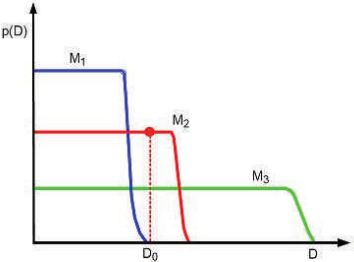
\includegraphics[scale=.80]{Bayesian-Occams-razor.png}
\caption{A schematic illustration of the Bayesian Occam’s razor. The broad (green) curve corresponds to a complex model, the narrow (blue) curve to a simple model, and the middle (red) curve is just right. Based on Figure 3.13 of (Bishop 2006a). }
\label{fig:Bayesian-Occams-razor} 
\end{figure}

When using the Bayesian approach, we are not restricted to evaluating the evidence at a finite grid of values. Instead, we can use numerical optimization to find $\lambda^*=\arg\max_{\lambda}p(\mathcal{D}|\lambda)$. This technique is called \textbf{empirical Bayes} or \textbf{type II maximum likelihood} (see Section \ref{sec:Empirical-Bayes} for details). An example is shown in Figure TODO(b): we see that the curve has a similar shape to the CV estimate, but it can be computed more efficiently.


\subsection{Computing the marginal likelihood (evidence)}
\label{sec:Computing-the-marginal-likelihood}
When discussing parameter inference for a fixed model, we often wrote
\begin{equation}
p(\vec{\theta}|\mathcal{D},m) \propto p(\vec{\theta}|m)p(\mathcal{D}|\vec{\theta},m)
\end{equation}
thus ignoring the normalization constant $p(\mathcal{D}|m)$. This is valid since $p(\mathcal{D}|m)$is constant wrt $\vec{\theta}$. However, when comparing models, we need to know how to compute the marginal likelihood, $p(\mathcal{D}|m)$. In general, this can be quite hard, since we have to integrate over all possible parameter values, but when we have a conjugate prior, it is easy to compute, as we now show.

Let $p(\vec{\theta})=q(\vec{\theta})/Z_0$ be our prior, where $q(\vec{\theta})$ is an unnormalized distribution, and $Z_0$ is the normalization constant of the prior. Let $p(\mathcal{D}|\vec{\theta})=q(\mathcal{D}|\vec{\theta})/Z_{\ell}$ be the likelihood, where $Z_{\ell}$ contains any constant factors in the likelihood. Finally let $p(\vec{\theta}|\mathcal{D})=q(\vec{\theta}|\mathcal{D})/Z_N$ be our posterior , where $q(\vec{\theta}|\mathcal{D})=q(\mathcal{D}|\vec{\theta})q(\vec{\theta})$ is the unnormalized posterior, and $Z_N$ is the normalization constant of the posterior. We have
\begin{align}
p(\vec{\theta}|\mathcal{D})& =\dfrac{p(\mathcal{D}|\vec{\theta})p(\vec{\theta})}{p(\mathcal{D})} \\
\dfrac{q(\vec{\theta}|\mathcal{D})}{Z_N}& =\dfrac{q(\mathcal{D}|\vec{\theta})q(\vec{\theta})}{Z_{\ell}Z_0p(\mathcal{D})} \\
p(\mathcal{D})& = \dfrac{Z_N}{Z_0Z_{\ell}}
\end{align}

So assuming the relevant normalization constants are tractable, we have an easy way to compute the marginal likelihood. We give some examples below.

\subsubsection{Beta-binomial model}
Let us apply the above result to the Beta-binomial model. Since we know $p(\vec{\theta}|\mathcal{D})=\mathrm{Beta}(\vec{\theta}|a',b')$, where $a'=a+N_1$, $b'=b+N_0$, we know the normalization constant of the posterior is $B(a',b')$. Hence
\begin{align}
p(\theta|\mathcal{D})& =\dfrac{p(\mathcal{D}|\theta)p(\theta)}{p(\mathcal{D})} \\
    & =\dfrac{1}{p(\mathcal{D})}\left[\dfrac{1}{B(a,b)}\theta^{a-1}(1-\theta)^{b-1}\right] \nonumber \\
	& \quad \left[\dbinom{N}{N_1}\theta^{N_1}(1-\theta)^{N_0}\right] \\
	& =\dbinom{N}{N_1}\dfrac{1}{p(\mathcal{D})}\dfrac{1}{B(a,b)}\left[\theta^{a+N_1-1}(1-\theta)^{b+N_0-1}\right]
\end{align}

So
\begin{align}
\dfrac{1}{B(a+N_1,b+N_0)} & = \dbinom{N}{N_1}\dfrac{1}{p(\mathcal{D})}\dfrac{1}{B(a,b)} \\
p(\mathcal{D}) & = \dbinom{N}{N_1}\dfrac{B(a+N_1,b+N_0)}{B(a,b)}
\end{align}

The marginal likelihood for the Beta-Bernoulli model is the same as above, except it is missingthe $\binom{N}{N_1}$ term.

\subsubsection{Dirichlet-multinoulli model}
By the same reasoning as the Beta-Bernoulli case, one can show that the marginal likelihood for the Dirichlet-multinoulli model is given by
\begin{align}
p(\mathcal{D}) & =\dfrac{B(\vec{N}+\vec{\alpha})}{B(\vec{\alpha})} \\
   & = \dfrac{\Gamma(\sum_k \alpha_k)}{\Gamma(N+\sum_k \alpha_k)}\prod\limits_k \dfrac{\Gamma(N_k+\alpha_k)}{\Gamma(\alpha_k)}
\end{align}

\subsubsection{Gaussian-Gaussian-Wishart model}
Consider the case of an MVN with a conjugate NIW prior. Let $Z_0$ be the normalizer for the prior, $Z_N$ be normalizer for the posterior, and let $Z_{\ell}(2\pi)^{ND/2}=$ be the normalizer for the likelihood. Then it is easy to see that
\begin{align}
p(\mathcal{D})& =\dfrac{Z_N}{Z_0Z_{\ell}} \\
   & = \dfrac{1}{(2\pi)^{ND/2}}\dfrac{\left(\frac{2\pi}{\kappa_N}\right)^{D/2}|\vec{S}_N|^{-\nu_N/2}2^{(\nu_0+N)D/2}\Gamma_D(\nu_N/2)}{\left(\frac{2\pi}{\kappa_0}\right)^{D/2}|\vec{S}_0|^{-\nu_0/2}2^{\nu_0D/2}\Gamma_D(\nu_0/2)} \\
   & = \dfrac{1}{\pi^{ND/2}}\left(\dfrac{\kappa_0}{\kappa_N}\right)^{D/2}\dfrac{|\vec{S}_0|^{\nu_0/2}}{|\vec{S}_N|^{\nu_N/2}}\dfrac{\Gamma_D(\nu_N/2)}{\Gamma_D(\nu_0/2)}
\end{align}

\subsubsection{BIC approximation to log marginal likelihood}
In general, computing the integral in Equation \ref{eqn:marginal-likelihood} can be quite difficult. One simple but popular approximation is known as the \textbf{Bayesian information criterion} or \textbf{BIC}, which has the following form (Schwarz 1978):
\begin{equation}
\mathrm{BIC} \triangleq \log p(\mathcal{D}|\hat{\vec{\theta}})-\dfrac{\mathrm{dof}(\hat{\vec{\theta}})}{2}\log{N}
\end{equation}
where $\mathrm{dof}(\hat{\vec{\theta}})$ is the number of \textbf{degrees of freedom} in the model, and $\hat{\vec{\theta}}$ is the MLE for the model. We see that this has the form of a \textbf{penalized log likelihood}, where the penalty term depends on the model’s complexity. See Section TODO for the derivation of the BIC score.

As an example, consider linear regression. As we show in Section TODO, the MLE is given by $\hat{\vec{w}}=(\vec{X}^T\vec{X})^{-1}\vec{X}^T\vec{y}$ and $\sigma^2=\frac{1}{N}\sum_{i=1}^N (y_i-\hat{\vec{w}}^T\vec{x}_i)$. The corresponding log likelihood is given by
\begin{equation}
\log p(\mathcal{D}|\hat{\vec{\theta}}) = -\dfrac{N}{2}\log(2\pi\hat{\sigma}^2)-\dfrac{N}{2}
\end{equation}

Hence the BIC score is as follows (dropping constant terms)
\begin{equation}
\mathrm{BIC}=-\dfrac{N}{2}\log(\hat{\sigma}^2)-\dfrac{D}{2}\log{N}
\end{equation}
where $D$ is the number of variables in the model. In the statistics literature, it is common to use an alternative definition of BIC, which we call the BIC \emph{cost}(since we want to minimize it):
\begin{equation}
\mathrm{BIC\text{-}cost} \triangleq -2\log p(\mathcal{D}|\hat{\vec{\theta}})-\mathrm{dof}(\hat{\vec{\theta}})\log{N} \approx -2\log{p(\mathcal{D})}
\end{equation}

In the context of linear regression, this becomes
\begin{equation}
\mathrm{BIC\text{-}cost} = N\log(\hat{\sigma}^2)+D\log{N}
\end{equation}

The BIC method is very closely related to the \textbf{minimum description length} or \textbf{MDL} principle, which characterizes the score for a model in terms of how well it fits the data, minus how complex the model is to define. See (Hansen and Yu 2001) for details.

There is a very similar expression to BIC/ MDL called the \textbf{Akaike information criterion} or \textbf{AIC}, defined as
\begin{equation}
\mathrm{AIC}(m,\mathcal{D}) = \log{p(\mathcal{D}|\hat{\vec{\theta}}_{MLE})}-\mathrm{dof}(m)
\end{equation}

This is derived from a frequentist framework, and cannot be interpreted as an approximation to the marginal likelihood. Nevertheless, the form of this expression is very similar to BIC. We see that the penalty for AIC is less than for BIC. This causes AIC to pick more complex models. However, this can result in better predictive accuracy. See e.g., (Clarke et al. 2009, sec 10.2) for further discussion on such information criteria.

\subsubsection{Effect of the prior}
Sometimes it is not clear how to set the prior. When we are performing posterior inference, the details of the prior may not matter too much, since the likelihood often overwhelms the prior anyway. But when computing the marginal likelihood, the prior plays a much more important role, since we are averaging the likelihood over all possible parameter settings, as weighted by the prior.

If the prior is unknown, the correct Bayesian procedure is to put a prior on the prior. If the prior is unknown, the correct Bayesian procedure is to put a prior on the prior. 


\subsection{Bayes factors}
Suppose our prior on models is uniform, $p(m) \propto 1$. Then model selection is equivalent to picking the model with the highest marginal likelihood. Now suppose we just have two models we are considering, call them the \textbf{null hypothesis}, $M_0$, and the \textbf{alternative hypothesis}, $M_1$. Define the \textbf{Bayes factor} as the ratio of marginal likelihoods:
\begin{equation}
\mathrm{BF}_{1,0} \triangleq \dfrac{p(\mathcal{D}|M_1)}{p(\mathcal{D}|M_0)}=\dfrac{p(M_1|\mathcal{D})}{p(M_2|\mathcal{D})}/\dfrac{p(M_1)}{p(M_0)}
\end{equation}


\section{Priors}
The most controversial aspect of Bayesian statistics is its reliance on priors. Bayesians argue this is unavoidable, since nobody is a \textbf{tabula rasa} or \textbf{blank slate}: all inference must be done conditional on certain assumptions about the world. Nevertheless, one might be interested in minimizing the impact of one’s prior assumptions. We briefly discuss some ways to do this below.


\subsection{Uninformative priors}
If we don’t have strong beliefs about what $\theta$ should be, it is common to use an \textbf{uninformative} or \textbf{non-informative} prior, and to “let the data speak for itself”.


\subsection{Robust priors}
In many cases, we are not very confident in our prior, so we want to make sure it does not have an undue influence on the result. This can be done by using \textbf{robust priors}(Insua and Ruggeri 2000), which typically have heavy tails, which avoids forcing things to be too close to the prior mean.


\subsection{Mixtures of conjugate priors}
Robust priors are useful, but can be computationally expensive to use. Conjugate priors simplify the computation, but are often not robust, and not flexible enough to encode our prior knowledge. However, it turns out that a \textbf{mixture of conjugate priors} is also conjugate, and can approximate any kind of prior (Dallal and Hall 1983; Diaconis and Ylvisaker 1985). Thus such priors provide a good compromise between computational convenience and flexibility.


\section{Hierarchical Bayes}
A key requirement for computing the posterior $p(\vec{\theta}|\mathcal{D})$ is the specification of a prior $p(\vec{\theta}|\vec{\eta})$, where $\vec{\eta}$ are the hyper-parameters. What if we don’t know how to set $\vec{\eta}$? In some cases, we can use uninformative priors, we we discussed above. A more Bayesian approach is to put a prior on our priors! In terms of graphical models (Chapter TODO), we can represent the situation as follows:
\begin{equation}
\vec{\eta} \rightarrow \vec{\theta} \rightarrow \mathcal{D}
\end{equation}

This is an example of a \textbf{hierarchical Bayesian model}, also called a \textbf{multi-level} model, since there are multiple levels of unknown quantities. 


\section{Empirical Bayes}
\label{sec:Empirical-Bayes}

\begin{table}
\centering
\begin{tabular}{ll}
\hline\noalign{\smallskip}
\textbf{Method} & \textbf{Definition} \\
\noalign{\smallskip}\svhline\noalign{\smallskip}
Maximum likelihood & $\hat{\vec{\theta}}=\arg\max_{\vec{\theta}} p(\mathcal{D}|\vec{\theta})$ \\
MAP estimation & $\hat{\vec{\theta}}=\arg\max_{\vec{\theta}} p(\mathcal{D}|\vec{\theta})p(\vec{\theta}|\vec{\eta})$ \\
\multirow{2}{*}{ML-II (\textbf{Empirical Bayes})} & $\hat{\vec{\eta}}=\arg\max_{\vec{\eta}} \int p(\mathcal{D}|\vec{\theta})p(\vec{\theta}|\vec{\eta})\mathrm{d}\vec{\theta}$ \\
                                                  & $\quad =\arg\max_{\vec{\eta}}p(\mathcal{D}|\vec{\eta})$ \\
\multirow{2}{*}{MAP-II} & $\hat{\vec{\eta}}=\arg\max_{\vec{\eta}} \int p(\mathcal{D}|\vec{\theta})p(\vec{\theta}|\vec{\eta})p(\vec{\eta})\mathrm{d}\vec{\theta}$ \\
                        & $\quad =\arg\max_{\vec{\eta}}p(\mathcal{D}|\vec{\eta})p(\vec{\eta})$ \\
Full Bayes & $p(\vec{\theta},\vec{\eta}|\mathcal{D}) \propto p(\mathcal{D}|\vec{\theta})p(\vec{\theta}|\vec{\eta})$ \\
\noalign{\smallskip}\hline
\end{tabular}
\end{table}


\section{Bayesian decision theory}
\label{sec:Bayesian-decision-theory}
We have seen how probability theory can be used to represent and updates our beliefs about the state of the world. However, ultimately our goal is to convert our beliefs into actions. In this section, we discuss the optimal way to do this.

Our goal is to devise a \textbf{decision procedure} or \textbf{policy}, $f(\vec{x}) : \mathcal{X} \rightarrow \mathcal{Y}$, which minimizes the \textbf{expected loss} $R_{\mathrm{exp}}(f)$(see Equation \ref{eqn:expected-loss}).

In the Bayesian approach to decision theory, the optimal output, having observed $\vec{x}$, is defined as the output $a$ that minimizes the \textbf{posterior expected loss}:
\begin{equation}
\rho(f)=\mathbb{E}_{p(y|\vec{x})}[L(y,f(\vec{x}))]=\begin{cases}
\sum\limits_y L[y,f(\vec{x})]p(y|\vec{x}) \\
\int\limits_y L[y,f(\vec{x})]p(y|\vec{x})\mathrm{d}y
\end{cases}
\end{equation}

Hence the \textbf{Bayes estimator}, also called the \textbf{Bayes decision rule}, is given by
\begin{equation}
\delta(\vec{x})=\arg\min\limits_{f \in \mathcal{H}} \rho(f)
\end{equation}


\subsection{Bayes estimators for common loss functions}


\subsubsection{MAP estimate minimizes 0-1 loss}
When $L(y,f(x))$ is \textbf{0-1 loss}(Section \ref{sec:Loss-function-and-risk-function}), we can proof that MAP estimate minimizes 0-1 loss, 
\begin{align*}
\arg\min\limits_{f \in \mathcal{H}} \rho(f)& =\arg\min\limits_{f \in \mathcal{H}} \sum\limits_{i=1}^K{L[C_k,f(\vec{x})]p(C_k|\vec{x})} \\
         & =\arg\min\limits_{f \in \mathcal{H}} \sum\limits_{i=1}^K{\mathbb{I}(f(\vec{x}) \neq C_k)p(C_k|\vec{x})} \\
		 & =\arg\min\limits_{f \in \mathcal{H}} \sum\limits_{i=1}^K{p(f(\vec{x}) \neq C_k|\vec{x})} \\
		 & =\arg\min\limits_{f \in \mathcal{H}} \left[1-{p(f(\vec{x}) = C_k|\vec{x})}\right] \\
		 & =\arg\max\limits_{f \in \mathcal{H}} p(f(\vec{x}) = C_k|\vec{x})
\end{align*}


\subsubsection{Posterior mean minimizes	$\ell_2$(quadratic) loss}
For continuous parameters, a more appropriate loss function is \textbf{squared error}, \textbf{$\ell_2$ loss}, or \textbf{quadratic loss}, defined as $L(y,f(\vec{x}))=\left[y-f(\vec{x})\right]^2$.

The posterior expected loss is given by
\begin{equation}\begin{split}
\rho(f) & =\int\limits_y L[y,f(\vec{x})]p(y|\vec{x})\mathrm{d}y \\
        & =\int\limits_y \left[y-f(\vec{x})\right]^2p(y|\vec{x})\mathrm{d}y \\
        & =\int\limits_y \left[y^2-2yf(\vec{x})+f(\vec{x})^2\right]p(y|\vec{x})\mathrm{d}y
\end{split}\end{equation}

Hence the optimal estimate is the posterior mean:
\begin{align}
& \dfrac{\partial \rho}{\partial f} =\int\limits_y [-2y+2f(\vec{x})]p(y|\vec{x})\mathrm{d}y=0 \Rightarrow \nonumber \\
& \int\limits_y f(\vec{x})p(y|\vec{x})\mathrm{d}y = \int\limits_y yp(y|\vec{x})\mathrm{d}y \nonumber \\
& f(\vec{x}) \int\limits_y p(y|\vec{x})\mathrm{d}y = \mathbb{E}_{p(y|\vec{x})}[y] \nonumber \\
& f(\vec{x}) = \mathbb{E}_{p(y|\vec{x})}[y]
\end{align}

This is often called the \textbf{minimum mean squared error} estimate or \textbf{MMSE} estimate.


\subsubsection{Posterior median minimizes $\ell_1$(absolute) loss}
The $\ell_2$ loss penalizes deviations from the truth quadratically, and thus is sensitive to outliers. A more robust alternative is the absolute or $\ell_1$ loss. The optimal estimate is the posterior median, i.e., a value $a$ such that $P(y<a|\vec{x})=P(y \geq a|\vec{x})=0.5$.

\begin{proof}
\begin{align*}
\rho(f)& =\int\limits_y L[y,f(\vec{x})]p(y|\vec{x})\mathrm{d}y=\int\limits_y |y-f(\vec{x})|p(y|\vec{x})\mathrm{d}y \\
       & =\int\limits_y [f(\vec{x})-y]p(y<f(\vec{x})|\vec{x})+ \\
	   & \quad [y-f(\vec{x})]p(y \geq f(\vec{x})|\vec{x})\mathrm{d}y \\
& \dfrac{\partial \rho}{\partial f}=\int\limits_y \left[p(y<f(\vec{x})|\vec{x})-p(y \geq f(\vec{x})|\vec{x})\right]\mathrm{d}y=0 \Rightarrow \\
& p(y<f(\vec{x})|\vec{x})=p(y \geq f(\vec{x})|\vec{x})=0.5 \\
& \therefore f(\vec{x})=\text{median}
\end{align*}
\end{proof}


\subsubsection{Reject option}
In classification problems where $p(y|\vec{x})$ is very uncertain, we may prefer to choose a reject action, in which we refuse to classify the example as any of the specified classes, and instead say “don’t know”. Such ambiguous cases can be handled by e.g., a human expert. This is useful in \textbf{risk averse} domains such as medicine and finance.

We can formalize the reject option as follows. Let choosing $f(\vec{x})=c_{K+1}$ correspond to picking the reject action, and choosing $f(\vec{x}) \in \{C_1,...,C_k\}$ correspond to picking one of the classes. Suppose we define the loss function as
\begin{equation}
L(f(\vec{x}), y)=\begin{cases} 
0 & \text{if } f(\vec{x})=y \text{ and } f(\vec{x}),y \in \{C_1,...,C_k\} \\
\lambda_s & \text{if } f(\vec{x}) \neq y \text{ and } f(\vec{x}),y \in \{C_1,...,C_k\} \\
\lambda_r & \text{if } f(\vec{x})=C_{K+1}
\end{cases}
\end{equation}
where $\lambda_s$ is the cost of a substitution error, and $\lambda_r$ is the cost of the reject action. 


\subsubsection{Supervised learning}
We can define the loss incurred by $f(\vec{x})$ (i.e., using this predictor) when the unknown state of nature is $\vec{\theta}$(the parameters of the data generating mechanism) as follows:
\begin{equation}
L(\vec{\theta},f) \triangleq \mathbb{E}_{p(\vec{x},y|\vec{\theta})}[\ell(y-f(\vec{x}))]
\end{equation}

This is known as the \textbf{generalization error}. Our goal is to minimize the posterior expected loss, given by
\begin{equation}
\rho(f|\mathcal{D}) = \int{p(\vec{\theta}|\mathcal{D})L(\vec{\theta},f)}\mathrm{d}\vec{\theta}
\end{equation}

This should be contrasted with the frequentist risk which is defined in Equation TODO.


\subsection{The false positive vs false negative tradeoff}
In this section, we focus on binary decision problems, such as hypothesis testing, two-class classification, object/ event detection, etc. There are two types of error we can make: a \textbf{false positive}(aka \textbf{false alarm}), or a \textbf{false negative}(aka \textbf{missed detection}). The 0-1 loss treats these two kinds of errors equivalently. However, we can consider the following more general loss matrix:

TODO
